\documentclass[paper=a4, fontsize=11pt]{scrartcl}

%\usepackage[T1]{fontenc} 
\usepackage[english]{babel} 
\usepackage{amsmath}
\usepackage{amsfonts}
\usepackage{amsthm}
\usepackage{amssymb}
\usepackage{changepage}
\usepackage{titlesec}
\usepackage{subcaption}
\usepackage{xspace}
\newcommand{\MATLAB}{\textsc{Matlab}\xspace}
\usepackage{sectsty} 
\usepackage{graphicx} 

\sectionfont{\centering \normalfont \scshape}
\subsectionfont{\normalfont}
\subsubsectionfont{\normalfont}

\usepackage{fancyhdr} 
\pagestyle{fancyplain} 
\fancyhead{} 
\fancyfoot[L]{} 
\fancyfoot[R]{} 
\fancyfoot[C]{\thepage} 
\renewcommand{\headrulewidth}{0pt} 
\renewcommand{\footrulewidth}{0pt} 
\setlength{\headheight}{13.6pt} 

\usepackage{enumitem}
\newcommand{\subscript}[2]{$#1 _ #2$}
\newcommand*\dif{\mathop{}\!\mathrm{d}}
\newcommand{\pder}[2]{\frac{\partial #1}{\partial #2}}   
\newcommand{\nextline}{$ $ \newline \vspace{-0.15in}}
\newcommand{\horrule}[1]{\rule{\linewidth}{#1}} 

\newcommand{\overbar}[1]{
	\mkern 1.5mu \overline{\mkern-1.5mu\raisebox{0pt}[\dimexpr\height+0.5mm\relax]{$#1$}\mkern-1.5mu}\mkern 1.5mu
}

%------------------------------
\title{	
	\normalfont \normalsize 
	\textsc{Konkuk University Dept. of Physics} \\ [25pt] %Konkuk University Dept. of Physics
	\horrule{1pt} \\[0.4cm] 
	\huge Numerical Analysis \\
	\vspace{0.1in}
	\Large 2019 Spring Semester
	\horrule{1pt} \\[0.4cm] 
}
\author{Youngwan Kim} 
\date{\normalsize\today} 
%------------------------------
\newtheorem{example}{Ex}
\newtheorem{theorem}{Thm}
\newtheorem{claim}{Claim}
\newtheorem*{remark}{Remark}
\newtheorem*{recall}{Recall}

\DeclareCaptionFont{white}{\color{white}}
\DeclareCaptionFormat{listing}{\colorbox{gray}{\parbox{\textwidth}{#1#2#3}}}
\captionsetup[lstlisting]{format=listing,labelfont=white,textfont=white}

%---------------------------------
\usepackage{listings}
\usepackage{inconsolata}
\usepackage{xcolor}
%\usepackage{courier}
\usepackage{color} %red, green, blue, yellow, cyan, magenta, black, white
\definecolor{mygreen}{RGB}{28,172,0} % color values Red, Green, Blue
\definecolor{mylilas}{RGB}{170,55,241}

\lstset{
	basicstyle=\ttfamily,
	language=Matlab,%
	%basicstyle=\color{red},
	breaklines=true,%
	morekeywords={matlab2tikz},
	keywordstyle=\color{blue},%
%	morekeywords=[2]{1}, keywordstyle=[2]{\color{black}},
%	identifierstyle=\color{black},%
	stringstyle=\color{mylilas},
	commentstyle=\color{mygreen},%
%	showstringspaces=false,%without this there will be a symbol in the places where there is a space
	numbers=left,%
	numberstyle={\tiny \color{black}},% size of the numbers
%	numbersep=5pt, % this defines how far the numbers are from the text
	emph=[1]{for,end,break},emphstyle=[1]\color{red}, %some words to emphasise
%	%emph=[2]{word1,word2}, emphstyle=[2]{style},   
}

%---------------------------------
\begin{document}
	
\maketitle	

\vspace{0.25in}

\section{Root Finding Methods}
\vspace{0.25in}
Finding roots for a given function in various situation can be considered as the very essential problem of numerical analysis. We introduce some root finding algorithms and apply it for finding solutions of a single variable equation, and if it is available we will also extend it for solving simultaneous equations. \\ 

\subsection{Bisection Method}
\vspace{0.15in}
The first method we introduce as a root finding algorithm is the bisection method. For a smooth function $f:I\subset\mathbb{R}\to \mathbb{R}$ which we need to get its roots, an interval $[a,b]\subset I$ is given where $f(a)f(b)<0$ which states that there is a zero point $p\in [a,b] : f(p) =0$. For such initial value given, we then :

\begin{enumerate}[label=\arabic*)]
	\item Get $a,b$ and $N,\epsilon$.
	\item Let $i=1$ and iterate until $i=N$
	\begin{enumerate}[label=(\arabic*)]
		\item Get $p=(a+b)/2$.
		\item if $f(p)=0$ or $f(p)<\epsilon$: break loop, output $p$
		\item if $f(p)f(a) >0$ : let $a=p$
		\item if $f(p)f(a) <0$ : let $b=p$
		\item $i=i+1$
	\end{enumerate}
	\item END \\
\end{enumerate}

The $\epsilon$ used here is the tolerance, the amount of error that we could tolerate. So unless the method fails to find a point which $f(p) < \epsilon$ even with $N$ iterations, the algorithm must stop at 2). The following \MATLAB code is an example depicting the application of bisection method where $f(x)=\cos(x)-x$ and the initial interval is given as $[0,\pi / 2]$.\\

\begin{lstlisting}[label=test.m,caption=bisec.m]
function bisec=bisec(n)

f=inline('cos(x)-x');
a=0; b=pi/2;
for k=1:n
  c=(a+b)/2;
   if(f(c)>0) a=c;  % we know that f(a)=f(0)>0 
   else b=c;
   end
end

fval=f(c)
\end{lstlisting}
\vspace{0.15in}

The code gets the iterating numbers as the only input and outputs the final value of $f(p)$, which is actually the error $|f(p)-0|$, without the sign. Also for the given function as we know the sign of $f(0)$, we slightly modified the comparing condition. The following output of $n=10,$ $50$ $,100$ shows that this method converges well if the inital value is given right.

\begin{verbatim}
octave:1> format long
octave:2> bisec(10)
fval = 0.00207533648652292
octave:3> bisec(50)
fval = 3.33066907387547e-16
octave:4> bisec(100)
fval = 0
\end{verbatim}

%Let us consider the convergence of the bisection method.

\subsection{Newton Method}
\vspace{0.15in}
\subsubsection{Single Value Equation : No Multiplicity}
\vspace{0.15in}
The previous bisection method was rather simple as an algorithm as it just used evaluation and comparision. The Newton method we introduce at this section uses the fact that \textbf{any function can be approximated linearly near any point}, which is the idea of differentiation, to find roots numerically. We can't assert the convergence of this method, compared to the bisection method which always converges to the root when right initial values were given, but when it converges it shows up to be a very efficient method, which means that it fastly converges to its root. Also this method requires differentiation of the given function, which is quite a computational burden, but we'll talk about it later. The algorithm goes like this :
\vspace{0.15in}

\begin{enumerate}[label=\arabic*)]
	\item Choose the initial point $x_0$.
	\item Let $i=1$ and iterate until $i=N$
	\begin{enumerate}[label=(\arabic*)]
		\item $x=x_0 - f(x_0)/f'(x_0)$
		\item if $|x-x_0|<\epsilon$ break loop ;
		\item let $x_0=x$
	\end{enumerate}
	\item  END\\
\end{enumerate}

The term $x_0 - f(x_0)/f'(x_0)$ is the gist of this method, which is derived from the linear approximation of $f(x)$ near $x_0$. For points near $x_0$,

\begin{equation}\nonumber
	\begin{split}
		f(x) &= f(x_0) + f'(x_0)(x-x_0)+ \frac{f''(\xi)}{2!}(x-x_0)^2 \\
		&\simeq f(x_0) + f'(x_0)(x-x_0)
	\end{split}
\end{equation}\\

where we ignored $\mathcal{O}((x-x_0)^2)$ terms and solving this for $x$ where $f(x)=0$ gives us 
\vspace{0.15in}
\begin{equation}\nonumber
x\simeq x_0 - \frac{f(x_0)}{f'(x_0)}
\end{equation}
\vspace{0.15in}

So we might question that \textit{" If this is method that great why don't we just find 'good' initial values that would eventually converge? "} for the non guranteed convergence that differs by the initial value of this method, but actually that question itself is also a very \textit{chaotic} problem. For instance we can extend this method for analytic functions $f:\mathbb{C}\to\mathbb{C}$, and the convergence of each points result in a fractal, where we call such fractal a \textbf{Newton fractal}. Nothing is strange about extending the method to complex functions, as \textbf{linear approximation is the main idea of the method}. This idea will be used again and again for many other cases, with multiple variables and so on.\\

The following \MATLAB code implements the Newton method to $f(x)=x^3 - 2ix -5 $ which is a complex function, $ f: \mathbb{C} \to \mathbb{C}$. We used $x_0=i$ as the initial value, and the single input to see how fast it converges.\\

\begin{lstlisting}[label=test.m,caption=newton1d.m]
function newton1d=newton1d(n)

f=inline('x.^3-2*i*x-5');
df=inline('3*x^2-2*i');

x=i;

for k=1:n
x1=x-f(x)/df(x);
x=x1;
end

fval=f(x)
\end{lstlisting}
\vspace{0.15in}

And the below is the outputs for quite low number of iterations, starting from absolutely no iteration $n=1$ to nearly 10 iterations. Note that the needed steps to approximately get to the point where $f(x) \sim 10^{-16}$ decreased remarkably compared to the case of bisection method which nearly needed 50 iterations.

\begin{verbatim}
octave:1> format long
octave:2> newton1d(1)
fval =  0.700955848884844 + 2.471552116522530i
octave:3> newton1d(5)
fval = -5.14255305006373e-12 - 9.24993415196695e-12i
octave:4> newton1d(10)
fval =  0.00000000000000e+00 + 2.22044604925031e-16i
\end{verbatim}

Now let us see how fast this method converges. We haven't explicitly shown it but the bisection method converged linearly, and now we will show that the Newton method converges quadratically. As we assumed no multiplicity of the root we will converge to, we can assume that $f(r)=0$ and $f'(r)=0$. Then for $f(r)$, we can expand it near the initial point $x_0$ as \\

\begin{equation}\nonumber
	0=f(r) \simeq f(x_0) + f'(x_0)(r-x_0) + \frac{f''(\xi)}{2!} (r-x_0)^2 \quad \text{where} \quad \exists\xi\in(r,x_0)
\end{equation}\\

and simplifying some terms, we derive :\\

\begin{equation}\nonumber
	x_0 - \frac{f(x_0)}{f'(x_0)} = r + \frac{f''(\xi)}{2f'(x_0)} (r-x_0)^2
\end{equation} \\

note that the LHS is the $x_1$ term of the Newton method so we can again simplify : \\

\begin{equation}\nonumber
		| x_1 - r | = \Bigg| \frac{f''(\xi)}{2f'(x_0)} \Bigg|  (r-x_0)^2 \leq M (r-x_0)^2
\end{equation}\\

which implies that the error $e_i=|r-x_i|$ will keep decrease, but in a quadratic sense as $e_1 \leq M {e_0}^2$. So for $\forall n \in \mathbb{N}$, we can say that $|x_{n+1}-r|\leq|x_n - r|^2$. This shows us that the Newton method converges quadratically, but as we stated before it has high dependence on the initial value which implies that this method isn't very stable.  \\

As we keep mention it let us see how the slight differences in initial values can result in a very unexpected variance to the convergence, and how out of grasp this kind of problem is for us. The following \MATLAB code \texttt{newton\_fractal.m} plots a Newton fractal for $f(x)=x^3-2x-5$. \\

To elaborate how this \texttt{newton\_fractal.m} works, it first starts by generating a $n \times n$ matrix, which can be thought as a lattice included in $\mathbb{C}$, the region where we want to plot the Newton fractal. In this case we assigned $n=250$, and the region to be $I\subset \mathbb{C}$ where $I=\{z\in\mathbb{C} : \Re(z)\in(-1.5,2.5) , \Im(z) \in (-1.5,1.5) \}$ which is specified in line \texttt{9}. Then for the main routine, each elements of the matrix will go through a Newton method routine and save a value differed by the value of the most adjacent root among the three known roots with the tolerance given $\epsilon \sim \mathcal{O}(10^{-6})$. Then after all the routines, we will obtain a $n \times n$ matrix filled with the values of $0,1,2$ and $3$. Note that not all values get assigned with $1,2,3$. We then use internal functions to plot the given matrix, which will be an approximate version -\textit{ low resolution version, I would say }- of the real Newton fractal structure. \\

\begin{lstlisting}[label=test.m,caption=newton\_fractal.m]
f=inline('x.^3-2*x-5');
df=inline('3*x^2-2');

xt(1)= 2.094551481542327;   
xt(2)=-1.047275740771163 + 1.135939889088928i;
xt(3)=-1.047275740771163 - 1.135939889088928i;
% three complex roots for f(x)

n=250; rx=linspace(-1.5,2.5,n); ix=linspace(-1.5,1.5,n);

z=zeros(n,n);

for m=1:n
 for j=1:n
  x=rx(m)+ix(j)*i;
   for k=1:25
    x=x-f(x)/df(x);
   end

  if(abs(x-xt(1))<10^(-6)) z(m,j)=1;
  elseif(abs(x-xt(2))<10^(-6)) z(m,j)=2;
  elseif(abs(x-xt(3))<10^(-6)) z(m,j)=3;
  end
 end
end

z=rot90(z);
figure; imagesc(z)
colormap([0 0 0; 1 0 0; 0 1 0; 0 0 1]) 
% each colors : black , R , G , B
\end{lstlisting}
\vspace{0.1in}

This code certainly has some heavy calculational complexity, approximately $\mathcal{O}(n^2)$ for the input value $n$, the wanted resolution of the Newton fractal plot. \\

\begin{figure}[htb]
\centering
\begin{subfigure}{0.25\textwidth}
	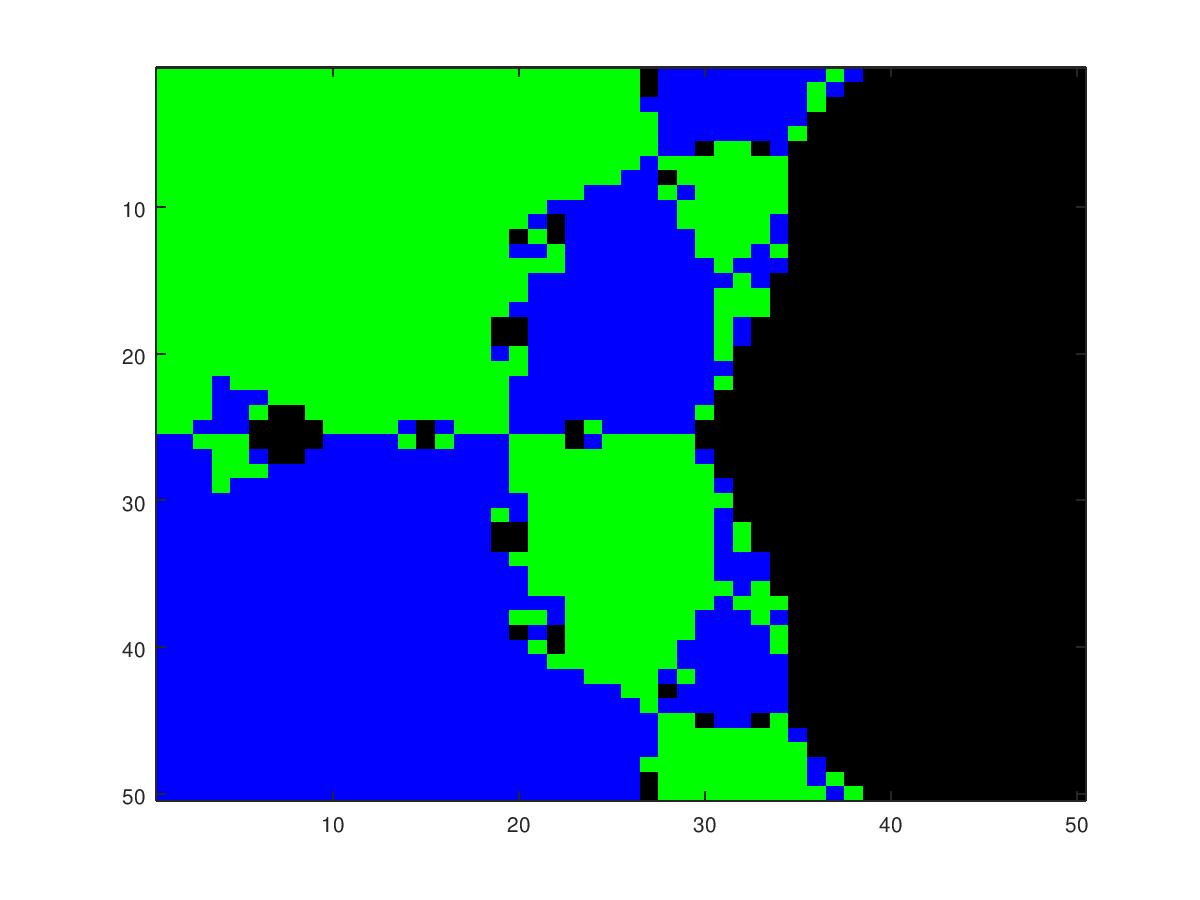
\includegraphics[width=\linewidth]{fractal_50}
	\caption{$n=50$}
\end{subfigure}\hfil % <-- added
\begin{subfigure}{0.25\textwidth}
	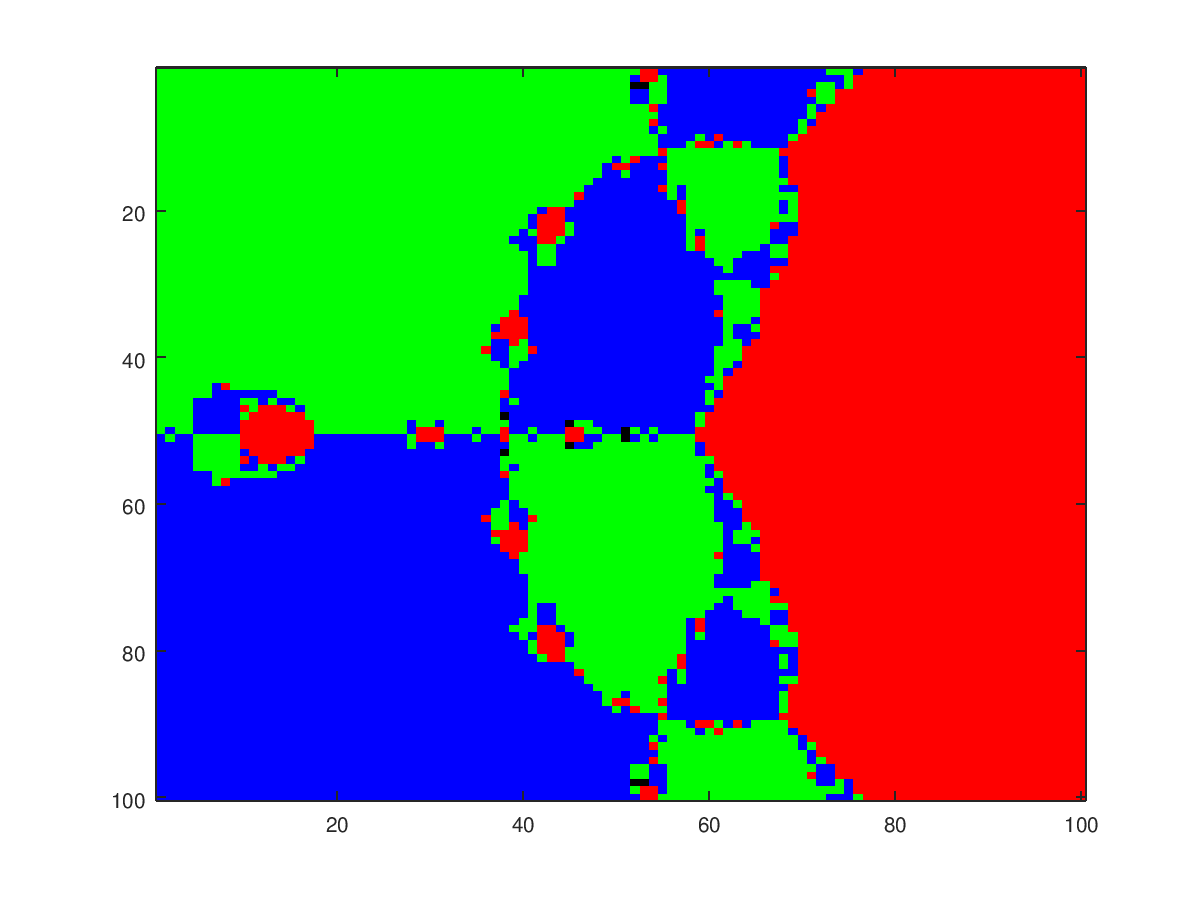
\includegraphics[width=\linewidth]{fractal_100}
	\caption{$n=100$}
\end{subfigure}\hfil % <-- added
\begin{subfigure}{0.25\textwidth}
	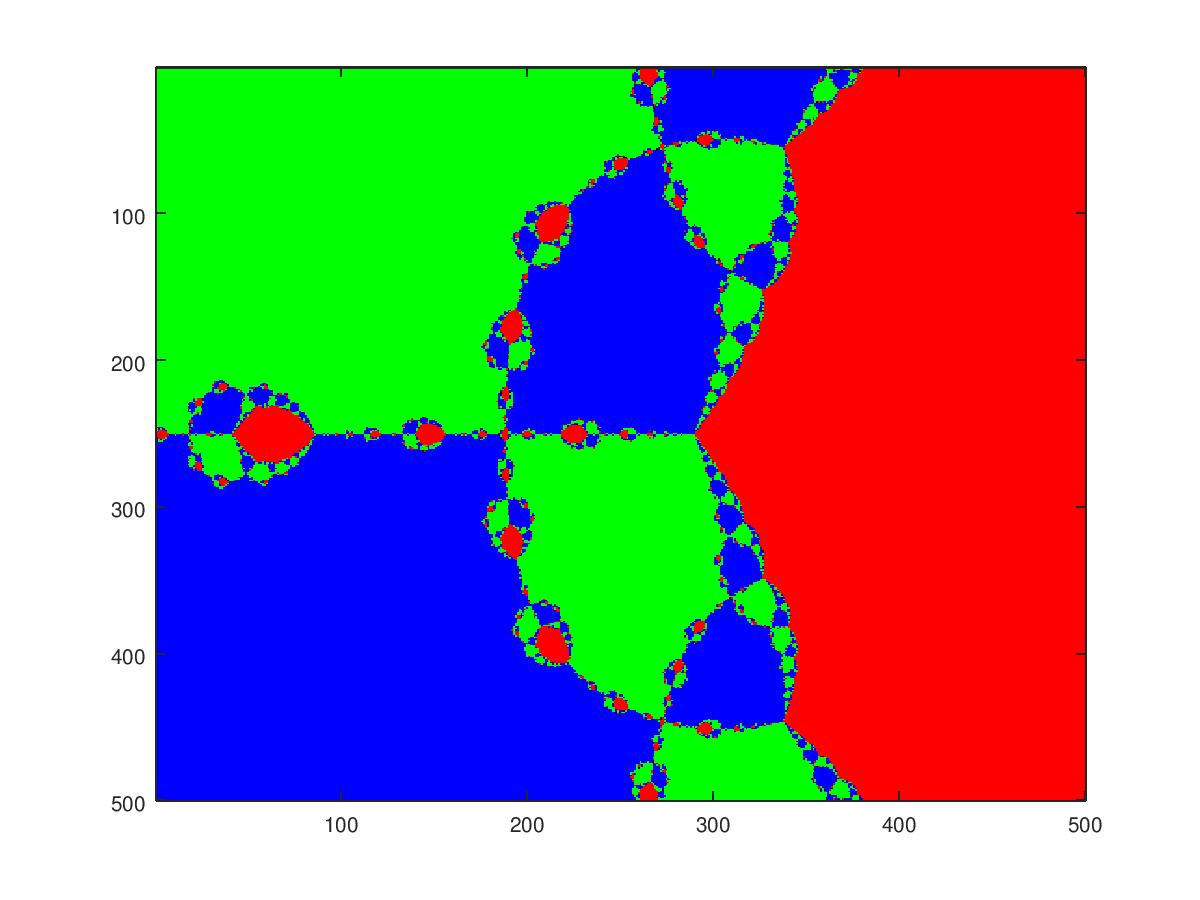
\includegraphics[width=\linewidth]{fractal_500_25}
	\caption{$n=500$}
\end{subfigure}
\end{figure}

\subsubsection{Two Variable Equations}
\vspace{0.15in}

We can extend this method to two variable problems. Let $f_1(x,y)$ and $f_2(x,y)$ be two variabled functions. We want to obtain $(x,y)$ such that $f_1(x,y)=0$ and $f_2(x,y)=0$ at the same time. Using the linear approximating idea of Newton method, we can design an algorithm as following :\\

\begin{enumerate}[label=\arabic*)]
	\item Get initial point $p_0=(x_0,y_0)$
	\item Let $i=1$ and iterate until given $N$ :
	\begin{enumerate}[label=(\arabic*)]
		\item The following equation \\
		\begin{equation}\nonumber
			p =
			\begin{pmatrix}
			 x \\ y
			\end{pmatrix}
			= 
			\begin{pmatrix}
			x_0 \\ y_0
			\end{pmatrix}
			-
			\begin{pmatrix}
			\partial_x f_1 & \partial_x f_2\\
			\partial_y f_1 & \partial_y f_2 
			\end{pmatrix}^{-1}_{p_0}
			\begin{pmatrix}
			f_1 \\ f_2
			\end{pmatrix}_{p_0}
		\end{equation}
		\item let $p_0=p$
		\item if $f_1(p) < \epsilon$ and $f_2(p) < \epsilon$ break loop;
	\end{enumerate}
	\item END \\
\end{enumerate} 

The equation is again derived by using linear approximations of $f_1$ and $f_2$. We'll let those approximated functions near $p_0$ as \\

\begin{equation}\nonumber
	\begin{cases}
	l_1 &= \partial_x f_1(p_0) (x-x_0)+ \partial_y f_1(p_0) (y-y_0) + f_1(p_0)\\
	l_2 &= \partial_x f_2(p_0) (x-x_0)+ \partial_y f_2(p_0) (y-y_0) + f_2(p_0) \\
	\end{cases}
\end{equation}\\

This approximation is available as $f_i(p_0)=l_i(p_0)$ and $\nabla f_i(p_0) = \nabla l_i (p_0)$ for all $i=1,2$. Thus we can reduce the problem of getting $(x,y) : f_1(x,y)=f_2(x,y)=0$ to a rather less complicated computation of finding $(x,y) : l_1(x,y) = l_2(x,y)=0$ between two linear functions.The following \MATLAB code is an example of applying the above method letting $f_1 = 2x^3 + y^3 +xy -6$ and $f_2 = x^3 - y^3 +xy -4$.\\

\begin{lstlisting}[label=test.m,caption=newton2d.m]
function newton2d=newton2d(n)

f=inline('[2*x^3+y^3+x*y-6; x^3-y^3+x*y-4]');
df=inline('[6*x^2+y 3*y^2+x; 3*x^2+y -3*y^2+x]');
x=[1 2]';

for k=1:n
 x=x-inv(df(x(1),x(2)))*f(x(1),x(2));
end

fval=f(x(1),x(2))'
\end{lstlisting}
\vspace{0.15in}

Again this gets a single input of amount of iteration, and outputs the final value after such number of iterations. The following is a set of outputs with $10$, $25$, and $50$ iterations.

\begin{verbatim}
octave:1> format long
octave:2> newton2d(10)
fval = 1.62917432964171e-03   5.71500960422355e-06
octave:3> newton2d(25)
fval = 8.88178419700125e-16   8.88178419700125e-16
octave:4> newton2d(50)
fval = 1.77635683940025e-15   0.00000000000000e+00

\end{verbatim}

\subsubsection{Single Variable Equations : Roots with Multiplicity}
\vspace{0.15in}

Not every case the Newton method acts fast, even if its convergence is guranteed. If a certain root has multiplicity, i.e $f(r)=f'(r)= \dots = f^{(m)}(r)=0$ the convergence is slower than when it has no multiplicity. So we tweak our Newton method for roots with multiplicity : when we know the exact multiplicity of a certain root, or else when we actually have no info about the multiplicity but only know that it is not a single root.\\

First let us start with the case where the multiplicity is unknown. We denote the multiplicity $m \geq 2$ of $r:f(r)=0$. Then, for some $g(x)$ such that $g(r)\neq 0$, \\

\begin{equation}\nonumber
	\begin{split}
	f(x) &= (x-r)^m g(x) \\[2.5ex]
	\implies \frac{f(x)}{f'(x)} &= \frac{(x-r)^m g(x)}{m (x-r)^{m-1} g(x) + (x-r)^m g'(x)} \\[2.5ex]
	&= (x-r) \left( \frac{g(x)}{mg(x)+(x-r)g'(x)} \right) \\
	\end{split}
\end{equation}\\

then this $f/f'$ has a simple root in $x=r$, which makes us available to apply Newton method. Then if we let $\{x_n\}$ be the Newton sequence of $f/f'$,\\

\begin{equation}\nonumber
	\begin{split}
	x_{n+1}&=x_n - \left( \frac{f(x_n)}{f'(x_n)} \right) \Big/ \left( \frac{f(x_n)}{f'(x_n)}  \right)' \\[2.5ex]
	& = x_n - \left( \frac{f}{f'} \right) \Big/ \left( \frac{f'f' - f f''}{f'^2}  \right) \\[2.5ex]
	&= x_n - \left( \frac{ff'}{f'^2 - ff''} \right)
	\end{split}
\end{equation}\\

would be the modified version for roots with unknown multiplicity. The Newton sequence has a second derivative, which isn't a very delightful situation as it brings us some calculational disadvantage. \\

Now we will consider the cases where the multiplicity is known, again we will let the multiplicity $m$, i.e, $f(r)=f'(r)= \cdots = f^{(m)}(r)=0$. This condition implies that $f^{(m-1)}(x)$ has $x=r$ as a single root. Then we will use the unmodified Newton method to $f^{(m-1)}(x)$. In this process, we use a useful approximation presented by Ralston \& Rabinowitz (1978), \\

\begin{equation}\nonumber
	\frac{f^{(m-1)}(x)}{f^{(m)}(x)} \simeq m \cdot \frac{f(x)}{f'(x)}
\end{equation} \\

As we claimed that we will apply Newton method to $f^{(m-1)}(x)$, let us consider the Newton sequence $\{x_n\}$ for it. Then, \\

\begin{equation}\nonumber
	\begin{split}
	x_{n+1} &= x_n - \frac{f^{(m-1)}(x)}{f^{(m)}(x)} \\[2.5ex]
	&\simeq x_n - m \frac{f(x)}{f'(x)} \qquad \text{[Ralston (1978)]}
	\end{split}
\end{equation}\\

becomes the Newton sequence to iterate, and thanks to the approximation of Ralston \& Rabinowitz we derived a method with no high computational disadvantage. We will show that this approximation works, by showing it has quadratic convergence. \\

First we can expand $f(x_n)$ around the root $x=r$, for $\exists \xi,\eta \in (r,x_n)$ :\\

\begin{equation}\nonumber
	\begin{split}
		f(x_n) &= \sum^{m-1}_{n=0} \frac{f^{(n)}(r)}{n!}(x_n-r)^n + \frac{f^{(m)}(\xi)}{m!}(x_n - r)^m  \\[2.5ex]
		&= \frac{f^{(m)}(\xi)}{m!}(x_n - r)^m \\[3.5ex]
		f'(x_n) &= \sum^{m-1}_{n=1} \frac{f^{(n)}(r)}{(n-1)!}(x_n-r)^{n-1} + \frac{f^{(m)}(\eta)}{(m-1)!}(x_n - r)^{m-1} \\[2.5ex]
		&= \frac{f^{(m)}(\eta)}{(m-1)!}(x_n - r)^{m-1} 
	\end{split}
\end{equation}\\

where we used the multiplicity condition to reduce terms. This implies that \\

\begin{equation}\nonumber
	\exists \eta,\xi \in (r,x_n) \quad : \quad m \frac{f(x_n)}{f'(x_n)} = \frac{f^{(m)}(\xi)}{f^{(m)}(\eta)} (x_n - r)
\end{equation}\\

Now we use the approximation of Ralson (1978) : \\

\begin{equation}\nonumber
	\begin{split}
	x_{n+1} = x_n - m \frac{f(x_n)}{f'(x_n)} &= x_n - \frac{f^{(m)}(\xi)}{f^{(m)}(\eta)} (x_n - r) \\[2.5ex]
	x_{n+1} -r &= (x_n - r) - \frac{f^{(m)}(\xi)}{f^{(m)}(\eta)} (x_n - r) \\[2.5ex]
	 &= (x_n - r)  \left[ 1- \frac{f^{(m)}(\xi)}{f^{(m)}(\eta)} \right] \\[2.5ex]
	 &= (x_n - r)  \left[ \frac{ f^{(m)}(\eta)- f^{(m)}(\xi)  }{f^{(m)}(\eta)}\right] \\[2.5ex]
	\exists \nu \in (r,x_n) \quad : \quad &\leq  (x_n - r) (\eta - \xi) \left[\frac{f^{(m+1)}(\nu)}{f^{(m)}(\eta)}\right]\\
	\end{split}
\end{equation}\\

And as $\exists \xi, \eta \in (r,x_n) \implies |\xi - \eta|\leq |x_n -r|$, and there exists some $M>0$ such that \\

\begin{equation}\nonumber
	| x_{n+1}-r | \leq M |x_n - r| |\eta - \xi|  \implies | x_{n+1}-r | \leq M |x_n - r|^2
\end{equation}\\

which implies that the error for such sequence quadratically converges to 0.\\

 Now we will use $f(x)=\sin^2(x)$ as an example which has multiplicity of 2 for its root $x=0$, and will apply all the three kinds of Newton method we introduced : the \textit{vanilla} Newton, the unknown multiplicity modification, and the Raston Newton method. We will compare the amount of time for each method to break the iteration with identical tolerance with $\epsilon\sim \mathcal{O}(10^{-15})$. We used the internal time function \texttt{tic} and \texttt{toc} of \MATLAB to measure how much time each methods used. Also for the initial value, we used the \texttt{rand} function, which outputs a random number in $(0,1)$. \\

\begin{lstlisting}[caption='newton\_modifications.m']
f=inline('sin(x)^2'); df=inline('sin(2*x)'); 
ddf=inline('2*cos(2*x)'); % for unknown multiplicity

x=rand;

tic 
for i=1:20 % Non-modified Newton
 x = x - f(x)/df(x);
 if(f(x) < 10^(-15)) break; end
end 
toc

tic 
for i=1:20 % Unknown multiplicity modification
 x = x - f(x)*df(x)/(df(x)*df(x)-f(x)*ddf(x));
 if(f(x) < 10^(-15)) break; end
end 
toc

tic 
for i=1:20 % Known multiplicity, Raston 1978 modification
 x=x-2*f(x)/df(x); % known multiplicity = 2  
 if(abs(df(x)) < 10^(-15)) break; end 
end 

\end{lstlisting}
\vspace{0.15in}

As we expected, the Raston-Newton method shows up to be the fastest method.

\begin{verbatim}
octave:1> format long
octave:2> newton_modifications
Elapsed time is 0.001894 seconds.
Elapsed time is 0.000106096 seconds.
Elapsed time is 5.00679e-05 seconds.
\end{verbatim}
\vspace{0.15in}

\subsection{Secant Method}
\vspace{0.15in}
The secant method is somehow a negotiation between the bisection and Newton method. It also uses linear approximation but not via the derivative concept. If the Newton method was using a single point to obtain the linear approximation of a certain function which can be thought of obtaining the instantaneous \textit{slope}, the secant method uses the fact that we can also approximate such instant derivative by substituting it with the slope of the secant line between necessarily adherent points. Thus it eases derivational burden for obtaining a linear approximation while getting a somehow reasonable accuracy, and at the same time gains stability better than the Newton method. \\

Let a function $f(x):\mathbb{R}\to\mathbb{R}$ with two given points as an initial value, let it $(x_0,f(x_0))$ and $(x_1, f(x_1))$. Then we approximate $f$ to a linear function $l(x): deg(l)=1$ which satisfies $f(x_0)=l(x_0)$ and $f(x_1)=l(x_1)$ at the same time. Obtaining such $l(x)$ is a quite elementary problem, \\

\begin{equation}\nonumber
	l(x) = \frac{f(x_0)-f(x_1)}{x_0 - x_1}(x-x_0)+ f(x_0)
\end{equation}\\

and we can easily show that it suffices the conditions we stated above. Using the root of this $l(x)$ we implement such algorithm :

\begin{enumerate}[label=\arabic*)]
	\item Get initial points $x_0,x_1$
	\item Let $i=0$ and iterate until $N$
	\begin{enumerate}[label=(\arabic*)]
		\item Get $x = x_0 - f(x_0)\frac{(x_0-x_1)}{f(x_0)-f(x_1)}$
		\item \texttt{temp}$= x_1$
		\item $x1=x$
		\item $x_0=$\texttt{temp}
		\item if $f(x)=0$ or $f(x) < \epsilon$ break loop;
	\end{enumerate}
	\item END
\end{enumerate} 

where we used a temporary variable \texttt{temp} to circulate the variables for the sequence to iterate through. The following \MATLAB code implemented the above algorithm where $f(x)=x^3-2x-5$ and the initial values are given as $x_0=0$ and $x_1=i$. \\

\begin{lstlisting}[caption = secant.m]
f=inline('x^3-2*x-5');

x0=0; x1=i;

for k=1:20
  x = x1 - f(x1)*(x0-x1)/(f(x0)-f(x1));
  temp=x1;
  x1=x;
  x0=temp;
  if(abs(f(x))<10^(-15)) break; end
  
iter = k

end

\end{lstlisting}
\vspace{0.15in}

Here we used $\epsilon \sim 10^{-15}$ as the tolerance for this algorithm. The output shows us how much iterations lead us to errors with $\epsilon$ tolerance. 

\begin{verbatim}
octave:1> secant
iter =  14
x = -1.04727574077116 + 1.13593988908893i
Elapsed time is 0.000838041 seconds.
\end{verbatim}

We can check that not even iterating until $k=20$, the loop broke at $k=14$. \\

Now we will calculate how this method converges towards the root. To recall, the bisection method had linear convergence, and the Newton method had quadratic convergence. To tell the results first, the secant method has $(1+\sqrt{5})/2$ convergence. Let us check how. \\

\begin{claim}
	$|x_2 - r| \leq M |x_1 - r | |x_0 - r|$
\end{claim}

\begin{proof}
	The secant method states that : \\
	
	\begin{equation}\nonumber
		x_2 = x_1 - \frac{f(x_1)(x_1 - x_0)}{f(x_1)-f(x_0)}
	\end{equation}\\
	
	which implies that \\
	
	\begin{equation}\nonumber
	\begin{split}
		x_2 - r &=  x_1 - \frac{f(x_1)(x_1 - x_0)}{f(x_1)-f(x_0)} -r \\[2.5ex]
		&= \frac{x_0 f(x_1) - x_1 f(x_0)}{f(x_1)-f(x_0)} -r \\[2.5ex]
		&= \frac{(x_0-r) f(x_1) - (x_1-r) f(x_0)}{f(x_1)-f(x_0)}  \\[2.5ex]
		&= \left(\frac{\frac{f(x_1)}{x_1 - r} - \frac{f(x_0)}{x_0 - r}}{f(x_1)-f(x_0)}\right) (x_0 -r)(x_1 - r)\\[2.5ex]
	\end{split}
	\end{equation}\\
	
	Thus to prove the \textbf{Claim 1} is identical of showing that the coefficient in front of $(x_0 -r)(x_1 - r)$ is bounded. Let $g(t) = f(t)/(t-r)$. Then, \\
	
	\begin{equation}\nonumber
		\begin{split}
		x_2 -r &= \frac{g(x_1)-g(x_0)}{f(x_1)-f(x_0)} (x_1 - r) (x_0 -r) \\[2.5ex]
		&= \frac{g'(\xi)}{f'(\xi)} (x_1 -r)(x_0 - r)
		\end{split}
	\end{equation}\\
	
	for some $\xi \in (x_0,x_1)$ due to Cauchy mean value theorem. We again use the Cauchy mean value theorem for $g'(\xi)$. By definition of $g(t)$ we explicitly get \\
	
	\begin{equation}\nonumber
		g'(\xi) = \frac{f'(\xi)(\xi - r) - f(\xi)}{(\xi - r )^2} = \frac{g_2(\xi)}{g_1(\xi)}
	\end{equation}\\
	
	where we let $g_2(\xi)= f'(\xi)(\xi - r) - f(\xi)$ and $g_1(\xi)=(\xi - r )^2$. For such $g_1,g_2$ we know that $g_1(r)=g_2(r)=0$ so we again apply Cauchy, for some $\zeta \in (\xi,r)$ \\
	
	\begin{equation}\nonumber
		\begin{split}
		g'(\xi) &= \frac{g_2(\xi)}{g_1(\xi)} = \frac{g_2(\xi) - g_2(r)}{g_1(\xi)- g_1(r)} = \frac{g_2'(\zeta)}{g_1'(\zeta)} \\[2.5ex]
		&= \frac{f''(\zeta)(\zeta - r)}{2(\zeta - r)} = \frac{1}{2} f''(\zeta)
		\end{split}
	\end{equation}\\
	
	Thus, the coefficient is bounded as \\
	
	\begin{equation}\nonumber
		\frac{g'(\xi)}{f'(\xi)} = \frac{f''(\zeta)}{2 f'(\xi)} \quad \text{ for } \quad ^\exists \xi \in (x_0,x_1)\text{ and } ^\exists\zeta \in (\xi,r) 
	\end{equation}\\
\end{proof}

Following the above method we can conclude that for any $n \in \mathbb{N}$, $|x_{n+2} - r| \leq M |x_{n+1} - r | |x_n - r| \implies e_{n+2} \leq M e_{n+1} e_{n}$ for some $M>0$. We then claim that\\

\begin{claim}
	$e_{n+1} \leq M e_n^{\frac{1+\sqrt{5}}{2}}$, where $e_i = |x_i -r|$.
\end{claim}

\begin{proof}
	Let $s=\max\{e_0,e_1\}$, which implies that $e_0 \leq s$ and also $e_1 \leq s$. Then using the relation $ e_{n+2} \leq  e_{n+1} e_{n}$ we can derive that $e_2 \leq s^2$. Doing this inductively, we get an inequality \\
	
	\begin{equation}\nonumber
		e_n \leq s^{\lambda_n} \quad \text{ where } \quad \lambda_{n+1} = \lambda_n + \lambda_{n-1} \quad (\lambda_0 = 0 \text{ , } \lambda_1 = 1) 
	\end{equation}\\
	
	with an exponential Fibonacci term. We know that we can express the general terms of $\lambda_n$ as \\
	
	\begin{equation}\nonumber
		\lambda_n = c_1 \left(\frac{1+\sqrt{5}}{2}\right)^n + c_2 \left(\frac{1-\sqrt{5}}{2}\right)^n  
	\end{equation}\\
	
	where we will denote $\frac{1+\sqrt{5}}{2}$ as $\alpha$ and the other one as $\beta$. Note that $\alpha + \beta = 1$ and $\alpha \beta = -1$. Then, \\
	
	\begin{equation}\nonumber
		e_{n+1} \leq  e_{n-1} e_{n} =  e_{n-1} e_{n}^{\alpha + \beta} = (e_{n-1} e_n^\beta) e_n^\alpha
	\end{equation}\\
	
	and we will show that $e_{n-1} e_n^\beta$ is bounded.\\
	
	\begin{equation} \nonumber
		\begin{split}
		 e_{n-1} e_n^\beta \leq s^{\lambda_{n-1}} s^{\beta \lambda_n} &= s^{c_1 \alpha^{n-1} + c_2 \beta^{n-1}} \cdot s^{\beta(c_1 \alpha^{n} + c_2 \beta^{n})}\\ 
		 &= s^{c_2(\beta^{n-1}+\beta^{n+1})} = s^{c_2 \beta^n(\beta^{-1}+\beta)}
		\end{split}
	\end{equation}\\
	
	As $|\beta| < 1$ , the $\beta_n$ term goes to 0 when $n \to \infty$, which implies that $ e_{n-1} e_n^\beta$ is bounded for some $N>0$. Thus, \\
	
	\begin{equation}\nonumber
		e_{n+1} \leq N e_n^\alpha = N e_n^{\frac{1+\sqrt{5}}{2}}
	\end{equation}\\
 \end{proof}

As $\alpha \simeq 1.62$, we can conclude that this method has efficiency somewhere between Newton $(n=2)$ and bisection $(n=1)$. Let's compare the convergence of all of the methods we introduced.\\

\begin{itemize}
	\item Bisection : $e_{n+1} \leq M e_n^1$ 
	\item Secant :  $e_{n+1} \leq M e_n^\frac{1+\sqrt{5}}{2} \simeq M e_n^{1.6} $ 
	\item Newton : $e_{n+1} \leq M e_n^2$ \\
\end{itemize}

Also do not forget about how to modify Newton method with functions with roots that have multiplicity, as regarding the multiplicity and modifying the method would enhance computation speed.

\vspace{0.25in}

\section{The Floating Number System}
\vspace{0.25in}

Numerical analysis is useful not because we know there exists a convergent series towards some root or value we need to derive, but rather there exists high speed computational machines that makes us available to implement such numerical algorithms, and finally output the value we want with very little error. So it is important to understand how the machines percieve real numbers, and how they process and save them as binary data.

\vspace{0.15in}

\subsection{IEEE 754 Standard}
\vspace{0.15in}

Most of the machine these days are 64-bit, so we will consider 64-bit real number representation, which means that for a real number we correspond an array of 64 binary numbers. The IEEE 754 standard for machine numbers is given as the following rule :\\

\begin{equation}\nonumber
	\underbar{$s$} \text{ } \underbar{$e_1 e_2 \cdots e_{11} $} \text{ }  \underbar{$b_1 b_2 \cdots b_{52} $}  = (-1)^{s} \cdot (1.b_1 b_2 \dots b_{52})_{(2)} \cdot 2^{(e_1 \cdots e_{11})_{(2)}-1023}
\end{equation} \\

where the first $s$ is the \textbf{sign indictor}, the following 11 digits are called the \textbf{characteristic} which denotes the exponent term, and the last 52 digits are called the \textbf{mantissa} which denotes the fractional term. 

This shows how different binary machines percieve real numbers compared to humans. The following \MATLAB code is a very good example showing such discrepancy.\\

\begin{lstlisting}[label=ridicule.m,caption=ridicule.m]
a=0;

for i=1:10
 a=a+0.1  
end

if (a==1) display('ok')
end
\end{lstlisting} 
\vspace{0.15in}

It is a rather simple code to understand : add 0.1 ten times, and if it is 1 print a string. Of course $10 \times 0.1 = 1$ for us, but the following result says that it isn't so for machines.

\begin{verbatim}
octave:1> ridicule
octave:2> 
\end{verbatim} 

This is because the representation of $0.1$ for binary machines doesn't actually represent the real number $0.1$. The following \MATLAB code is implemented to show the 64-bit representation of the input value.\\

\begin{lstlisting}[label=printmem, caption=print\_memory.m]
function [total64bits,sign,exponent,mantissa]=print_memory(x)

s = sprintf('%bx',x);
s = reshape(dec2bin(hex2dec(s'),4)',1,4*16);

total64bits=s;
sign=s(1:1);
exponent=s(2:12);
mantissa=s(13:end);
\end{lstlisting}
\vspace{0.15in}

Now using the above code let us speculate what happened in the perspective of the machine.

\begin{verbatim}
octave:1> print_memory(a)
ans = 0011111111101111111111111111111111111111111111111111111111111111
octave:2> print_memory(1)
ans = 0011111111110000000000000000000000000000000000000000000000000000
octave:3> print_memory(0.1)
ans = 0011111110111001100110011001100110011001100110011001100110011010
\end{verbatim}

We can check that $a=0.1 + \dots + 0.1$ is not percieved as 1 for binary machines, but rather a slightly smaller value than 1.  \\
 
We also need to consider which representations will correspond to $\infty$ and $0$, or in other words we need to assign certain boundaries for \textit{very small} and \textit{very big} numbers. We define the smallest number representation as \texttt{realmin} and the bigest number representation as \texttt{realmax}. To elaborate, we let $s=0$, $e=1$, and $b=0$ for \texttt{realmin} ,\\

\begin{equation}\nonumber
	\texttt{realmin} = 2^{-1022} \cdot (1.0) \sim 0.22 \times 10^{-307}
\end{equation}\\

and for representations between 0 and \texttt{realmin} we call it \textbf{underflow} and let all of it represent $0 \in \mathbb{R}$. For \texttt{realmax} we let $s=0$, $e=2046$, and $b=1-2^{-52}$,\\

\begin{equation}\nonumber
	\texttt{realmax} = 2^{1023} \cdot (2 - 2^{-52}) \sim 0.17 \times 10^{309}
\end{equation}\\

and for representations between \texttt{realmax} and \texttt{inf} we call it \textbf{overflow} and let all of it represent as a breaking point value for programs. Again using \texttt{print\_memory.m}, we explicitly see the 64-bit representation for \texttt{realmax},\texttt{realmin},\texttt{inf}, and 0.

\vspace{0.15in}
\begin{verbatim}
octave:1> print_memory(realmin)
ans = 0000000000010000000000000000000000000000000000000000000000000000
octave:2> print_memory(0)
ans = 0000000000000000000000000000000000000000000000000000000000000000
octave:3> print_memory(realmax)
ans = 0111111111101111111111111111111111111111111111111111111111111111
octave:3> print_memory(inf)
ans = 0111111111110000000000000000000000000000000000000000000000000000
\end{verbatim}
\vspace{0.15in}

The \texttt{IEEE 754} Standard representation is very useful, for two main reasons. It has a very wide range of real numbers available to represent, and also has a very small amount of relative error. To see how small the relative error is, consider two floating numbers\\

\begin{equation}\nonumber
\begin{split}
	\texttt{x1} &= (1.b_1b_2\dots b_{51} b_{52})_{(2)} \times 2^d  \\
	\texttt{x2} &= (1.b_1b_2\dots b_{51} 0)_{(2)} \times 2^d
\end{split}
\end{equation}\\

Then the relative error $\epsilon$ is, \\

\begin{equation}\nonumber
	\epsilon = \frac{(0.0\dots0b_{52})_{(2)} \cdot 2^d}{(1.b_1\dots b_{51}b_{52})_{(2)} \cdot 2^d} \leq 2^{-52}
\end{equation}\\

Thus the relative error has a magnitude of $2^{-52}$, which is really small. We can't make the full set of $\mathbb{R}$ to be percieved by machines which only speaks with 64 binary digits, but the double precision method is a way at least we can make them understand $\mathbb{R}$ as a set of numbers with very dense intervals between them, for a very large range.

\vspace{0.15in}

\subsection{Division Algorithm}
\vspace{0.15in}

For machines, understanding operations except addition and subtraction is quite a hard task to do. Subtraction and multiplication  between floating numbers can be implemented by modifying the addition method, and it is the best we can do. But think of multiplying a floating number by another one.  A process of getting an inverse of a certain floating number gets involved, which makes it very complicated. So the very problem of divising floating numbers eventually boils down to a problem of deriving inverses of $1\leq b <2$. \\

We know one way to find an inverse $b^{-1}$ of some floating number $b$ \textit{numerically}, if we regard it as a root of the function $f(x)=b-1/x$. As we know how this function looks like, without considering the initial value dependent stability of the Newton method, we can implement a quadratically converging algorithm of deriving inverse numbers. Also the derivation of the function $f(x)$ can be pre-calculated before plugging it into the algorithm, which also eases a step of computational burden of calculating the derivative of $f$.\\

Consider the Newton sequence $\{x_n\}$ for such $f(x)$, \\

\begin{equation}\nonumber
\begin{split}
		x_{n+1} &= x_n - \frac{f(x_n)}{f'(x_n)} = x_n - \left( \frac{b- 1/x_n}{1/x_n^2}\right) \\[1.5ex]
		&= x_n - (bx_n^2 -x_n) = 2x_n - bx_n^2
\end{split}
\end{equation}\\

we will set the initial value $x_0=3/4$ as $1\leq b <2$ we can assert convergence in this region - as it holds bisection conditions, a root must be there. Letting such initial value we can derive that the initial error has its maximum around $1/4$, and as the error converges quadratically we can have certainty that the method will let us converge real close to the real value.

\vspace{0.15in}
\begin{lstlisting}[caption=division.m]
function division=division(n) 
b=sqrt(2); % 1 < sqrt(2) < 2
x=3/4; err=0;

for k=1:n
 x=2*x-b*x*x ; % Newton sequence iteration
end
err=abs(x-1/b)
\end{lstlisting}
\vspace{0.15in}

The above \MATLAB code is the implementation of the division algorithm we introduced. It fastly converges to the real value, and the following output shows it :

\begin{verbatim}
octave:1> format long
octave:2> division(1)
err =  0.00260191002141352
octave:3> division(2)
err =  9.57413496749382e-06
octave:4> division(5)
err = 0
\end{verbatim}

\vspace{0.15in}

\section{Polynomials}
\vspace{0.25in}

The main goal of this section is to \textit{interpolate} polynomials, which is to construct new data from discrete given values. If we have $n$ points to interpolate, the result would be a $deg(p) < n$ polynomial $p$. For instance, consider a following situation where we need to construct a polynomial $p$ from a given data, let it $(x_i,p(x_i))$ for $i=1,2,3,4$. The simplest way to perform this is to let \\

\begin{equation}\nonumber
	p(x) = ax^3 + bx^2 + c^x + d 
\end{equation}\\

and get the coefficients by solving \\

\begin{equation}\nonumber
	\begin{pmatrix}
	x_1^3 & x_1^2 & x_1^1 & x_1^0 \\
	x_2^3 & x_2^2 & x_2^1 & x_2^0 \\
	x_3^3 & x_3^2 & x_3^1 & x_3^0 \\
	x_4^3 & x_4^2 & x_4^1 & x_4^0 \\
	\end{pmatrix}
	\begin{pmatrix}
	a \\ b\\ c \\ d\\
	\end{pmatrix}
	=
	\begin{pmatrix}
	p(x_1) \\ p(x_2) \\ p(x_3) \\ p(x_4)
	\end{pmatrix}
\end{equation}\\

which is a matrix equation, which we need to calculate an inverse. Such matrix is called a \textbf{Vandermonde matrix}, and \MATLAB has an internal function \texttt{vander} which calculates it. The following script is an example of calculating the coefficients of the interpolated polynomials for $(1,\log(1))$, $(2,\log(2))$, $(3,\log(3))$, and $(4,\log(4))$.

\begin{verbatim}
octave:1> v = [1 2 3 4] ;
octave:2> c = vander(v) \ log(v)' ;
octave:3> c'
ans = 0.028317  -0.313740   1.436152  -1.150728
\end{verbatim}

Certainly this requires high computational power as matrix inversion of a $n \times n$ matrix has complexity at least of $\mathcal{O}(n^{2.373})$ with optimized CW-like algorithms, or $\mathcal{O}(n^3)$ with the well known Gauss-Jordan elimination. Thus we introduce various polynomial interpolation methods from now on. Before interpolation methods, we introduce polynomial evaluation methods first, as we will use them later again and again.
\vspace{0.15in}
\subsection{Polynomial Evaluation}
\vspace{0.15in}
Evaluating polynomials is to get $p(x_0)$ for some $x_0$. Evaluation might seem simple, but as polynomials are linear combinations of different powers, and when the degree gets bigger, sometimes it requires a big amount of computation just to evaluate by \textit{brute forcing}, i.e, by direct calculation. \\

Consider a polynomial $p(x)$ with $deg(p)=n$. Evaluating such polynomial with direct calculation has at most $\mathcal{O}(n^2)$. A simple way to ease this is to use the memory property of machines, where we save $x_0^i$ as \texttt{v(i)} for some variable and then do the summation later. But during the saving process, again at most $\mathcal{O}(n^2)$ complexity is required.\\

 Thus we use \textbf{Horner's method} for evaluating polynomials. Any polynomial can be expressed in its \textbf{nested form}, for instance let $deg(p)=4$ then \\
 
 \begin{equation}\nonumber
 	p(x) = ax^4 + bx^3 + cx^2 + dx +e = \left( \left(\left(\left(x+a\right)x+b\right)x+c\right)x +d\right)x + e
 \end{equation}\\
 
 which can be applied to any kind of polynomials. The main point is that there is only $n$ times of multiplication occured in this method, reducing the complexity of evaluation which was at most $\mathcal{O}(n^2)$ to at most $\mathcal{O}(n)$. We will use this evaluation method very often. The following \MATLAB code depicts such method.\\

\begin{lstlisting}[caption='horner.m']
function horner_real=horner_real(c,x)
y=x+c(size(c,2))

for k=size(c,2)-1:-1:1
 y=y*x+c(k) 
end

\end{lstlisting}

 
\vspace{0.15in}
\subsection{Polynomial Interpolation}
\vspace{0.15in}

For a given $n+1$ distinct points $\{x_k\}_{k=0}^n$, the interpolation problem is to find the unique polynomial $P(x)$ with $deg(P) \leq n$, such that for a function $f(x)$ the following holds : \\

\begin{equation}\nonumber
	P(x_i) = f(x_i) \quad \text{for} \quad \forall i = 1,2 , \dots n
\end{equation}\\

We will introduce two interpolation methods, Lagrange and Newton. 

\vspace{0.15in}
\subsubsection{Lagrange Form}
\vspace{0.15in}
Let $L_k(x)$ be a polynomial as :\\

\begin{equation}\nonumber
	L_k(x) = \frac{(x - x_0)(x - x_1) \cdots (x - x_{k-1})(x - x_{k+1}) \cdots (x - x_n)}{(x_k - x_0)(x_k - x_1) \cdots (x_k - x_{k-1})(x_k - x_{k+1}) \cdots (x_k - x_n)}
\end{equation}\\

which also satisfies $L_k(x_i) = \delta_{ik}$. We can see that $deg(L_k) = n$ for any $L_k$. Now we define our interpolated result $P(x)$ as :\\

\begin{equation}\nonumber
	P(x) = \sum^{n}_{k=0} f(x_k) L_k(x)
\end{equation}\\

which has $deg(P) \leq n$. This method also requires a lot of computation.\\

\vspace{0.15in}
\subsubsection{Newton Form}
\vspace{0.15in}
The first step of this method is to let our interpolation $P(x)$ in such form :\\

\begin{equation}\nonumber
	P(x) = a_0 + a_1 (x-x_0)+  \cdots + a_n (x-x_0)(x-x_1) \cdots (x-x_{n-1})
\end{equation}\\

And we follow such recursive method to get the coefficients $\{a_i\}$.\\

\begin{enumerate}[label=(\arabic*)]
	\item $P_0(x)=f(x_0)$
	\item $P_1(x)=P_0(x)+a_1 (x-x_0) \text{ , } P_1(x_1) = f(x_1) $
	\vskip 0.5ex $\implies a_1 = (f(x_1) - P_0(x_1))/(x_1 - x_0)$
	\item $P_2(x)=P_1(x)+a_2 (x-x_0)(x-x_1) \text{ , } P_2(x_2) = f(x_2) $
	\vskip 0.5ex $\implies a_2 = (f(x_2) - P_1(x_2))/(x_2 - x_0)(x_2 - x_1)$ 
	\item $P_3(x)=P_2(x)+a_3 (x-x_0)(x-x_1)(x-x_2) \text{ , } P_3(x_3) = f(x_3) $
	\vskip 0.5ex $\implies a_3 = (f(x_3) - P_2(x_3))/(x_3 - x_0)(x_3 - x_1)(x_3 - x_2)$
	\\
	\vdots \\
\end{enumerate}

Where the each evaluation of $P_i(x_i)$ is implemented by Horner's method to minimize computation. Then generalizing the coefficient with step $j$, we get \\

\begin{equation} \nonumber
	a_j = \frac{f(x_j) - P_{j-1}(x_j)}{(x_j - x_0)(x_j - x_1) \cdots (x_j - x_{j-1})}
\end{equation}\\

From the above relation, we can implement a \MATLAB code which will input interpolation points, and evaluate a value for the interpolated polynomial. We will define two functions, one is the \texttt{horner(c,p,x)} function which will be used to evaluate a polynomial with Horner's method and the main \texttt{newton(p,v,x)} function.\\

\begin{lstlisting}[caption='newton\_horner.m']
function y=newton_horner(c,p,x) 

y=c(size(c,2)); 

for k = size(c,2)-1:-1:1 
 y = y*(x-p(k))+c(k);
end
\end{lstlisting}
\vspace{0.15in}

This Horner's method is slightly modified in order to directly apply to the Newton form we introduced, thus it needs another vector like variable \texttt{p} which denotes the $x_0,x_i \cdots x_{n-1}$ from the Newton form. The other variable \texttt{c} is also a vector input for the coefficients of a polynomial, and \texttt{x} is a scalar input to denote the point to evaluate the Newton form. This will act as a subroutine for our main \texttt{newton(p,v,x)} function. \\

\begin{lstlisting}[caption = 'newton.m']
function y=newton(p,v,x)
c=v(1);

for i=2:1:size(p,2)
 Q = 1;
  for m=1:1:i-1
   Q = Q*(p(i)-p(m));
  end
 c(i) = (v(i) - newton_horner(c,p,p(i))) / Q ;
end

y=newton_horner(c,p,x)
\end{lstlisting}
\vspace{0.15in}

The function \texttt{newton(p,v,x)} gets two $n$ vectors \texttt{p} and \texttt{v}, and a scalar \texttt{x} as an input, which each denotes an array of the interpolation points $x_i$ and interpolation values $P(x_i)$ and the point to evaluate the resulting interpolation. Using the routine we introduced, it gets the coefficients and save it as a vector \texttt{c}. We can see that during such routine the modified Horner evaluation \texttt{horner(c,p,p(i))} is used. After fully obtaining \texttt{c}, we then evaluate the value of $P(x)$ using \texttt{horner(c,p,x)} which is the final output of \texttt{newton(p,v,x)}. 

\vspace{0.15in}
\subsubsection{Interpolation Error}
\vspace{0.15in}

For the previous interpolation problem, now let us consider the error at a certain point $x$ which is $|f(x)-P(x)|$, we claim that : \\

\begin{claim}
For the unique interpolation $P(x)$ of $f(x)$ where $deg(P) \leq n$, there exists $\xi$ such that\\

\begin{equation}\nonumber
	f(x)-P(x) = \frac{f^{(n+1)}(\xi)}{(n+1)!} (x-x_0)(x-x_1) \cdots (x-x_n)
\end{equation}\\

where $\xi$ exists in $\min\{x_0, x_1, \dots , x_n\} < \xi < \max\{ x_0, x_1, \dots , x_n \}$.
\end{claim}

\begin{proof}
	Let $x \neq x_k$ for any $k=0,1,\dots n$ and define \\
	
	\begin{equation}\nonumber
		K = \frac{f(x)-P(x)}{(x-x_0)(x-x_1) \cdots (x-x_n)}
	\end{equation}\\
	
	Consider a function $g:\mathbb{R} \to \mathbb{R}$ as \\
	
	\begin{equation}\nonumber
		g(t) = f(t) - P(t) - K (t-x_0)(t-x_1) \cdots (t-x_n)
	\end{equation}\\
	
	then $g(x)=0$ and $g(x_k)=0$ for $k=0,1, \dots n$, which implies that $g$ vanishes at $n+2$ distinct points, and applying the mean value theorem recursively, there $^\exists \xi : \min\{x_0, x_1, \dots , x_n\} < \xi < \max\{ x_0, x_1, \dots , x_n \}$ such that \\
	
	\begin{equation}\nonumber
		g^{(n+1)}(\xi) = 0
	\end{equation}\\
	
	and by definition of $g(t)$,\\
	
	\begin{equation}\nonumber
	\begin{split}
		g^{(n+1)}(\xi) &= f^{(n+1)}(\xi) - P^{(n+1)}(\xi) - K \frac{d^{n+1}}{dt^{n+1}}(t-x_0)(t-x_1) \cdots (t-x_n) \Big|_{t = \xi} \\[2.5ex]
		&= f^{(n+1)}(\xi) - K (n+1)! =0
	\end{split}
	\end{equation}\\
	
	where we erased $P^{(n+1)}(\xi)$ as we know that $deg(P) \leq n$, and thus we can conclude that\\
	
	\begin{equation}\nonumber
	K = \frac{f(x)-P(x)}{(x-x_0)(x-x_1) \cdots (x-x_n)} = \frac{f^{(n+1)}(\xi) }{(n+1)!}
	\end{equation}\\
	
	for some $\xi$.\\
\end{proof}

\begin{example}
Some cases of considering interpolation errors, let $\epsilon(x)=f(x)-P(x)$ :\\
\begin{enumerate}[label=(\arabic*)]
	\item $f(a)=P(a), f'(a)=P'(a)$ and $f(b)=P(b)$, $f(c)=P(c)$.
	\vskip 1.5ex
	$\implies \epsilon(x) = \frac{f^{(4)}(\xi)}{4!}(x-a)^2(x-b)(x-c)$
	\item $f(a)=P(a), f'(a)=P'(a), f''(a)=P''(a)$ and $f(b)=P(b)$.
	\vskip 1.5ex
	$\implies \epsilon(x) = \frac{f^{(4)}(\xi)}{4!}(x-a)^3(x-b)$
	\item $f(a)=P(a), f'(a)=P'(a), f''(a)=P''(a),f'''(a)=P'''(a)$.
	\vskip 1.5ex
	$\implies \epsilon(x) = \frac{f^{(4)}(\xi)}{4!}(x-a)^4$
	
\end{enumerate}
\end{example}

\vspace{0.15in}
\subsection{Integration Methods}
\vspace{0.15in}

Using the interpolation methods and the concept of interpolation we've introduced we can numerically evaluate definite integrations of certain functions by \textit{slicing} the interval we want to integrate, and interpolating each intervals as polynomials with certain degrees that will differ by the various methods we will introduce. For the following, we will denote $f:[a,b]\to\mathbb{R}$ and $m=\frac{a+b}{2}$.

\vspace{0.15in}
\subsubsection{Trapezoidal Rule}
\vspace{0.15in}

Trapezoidal rule, as it name states is to interpolate the sliced intervals as trapezoidals, or to interpolate the function in the interval as a simple line between to points. We claim that certain approximation has cubic error respect to the size of the slice we chop up the interval.\\

\begin{claim}
	Let $T(f)$ be a functional of $f$ such that \\
	
	\begin{equation}\nonumber
		T(f) = (b-a)\frac{f(a)+f(b)}{2}
	\end{equation}\\
	
	Then the following holds : \\
	
	\begin{equation}\nonumber
		\left|\int_{a}^{b} f(x) \dif x  - T(f) \right| \leq \frac{1}{12} \max_{a\leq\xi\leq b} f''(\xi)(b-a)^3
	\end{equation}\\
\end{claim}

\begin{proof}
	First we interpolate using $(a,f(a))$ and $(b,f(b))$ which will result into a $deg(p) \leq 1$ polynomial. Then for such interpolation $p(x)$, $p(a)=f(a)$ and $p(b)=f(b)$ holds, which implies that \\
	
	\begin{equation}\nonumber
		T(f) = \int_{a}^{b} p(x) \dif x
	\end{equation}\\
	
	and for $^\forall t \in [a,b]$ and $^\exists \xi \in [a,b]$,\\
	
	\begin{equation}\nonumber
		f(t)-p(t) = \frac{f''(\xi)}{2!}(t-a)(t-b)
	\end{equation}\\
	
	which is the interpolation error of $p(x)$, and using this relation we can derive :\\
	
	\begin{equation}\nonumber
		\begin{split}
		\left|\int_{a}^{b} f(t) \dif t  - T(f) \right| &= \left|\int_{a}^{b} (f(t) - p(t)) \dif t \right| \\[2.5ex]
		&= \left|\int_{a}^{b} \frac{f''(\xi)}{2!}(t-a)(t-b)\dif t \right| \\[2.5ex]
		&\leq \frac{1}{2}  \max_{a\leq\xi\leq b} f''(\xi) \int_{a}^{b} \left|(t-a)(t-b) \right| \dif t \\[2.5ex]
		&= \frac{1}{12} \max_{a\leq\xi\leq b} f''(\xi)(b-a)^3 
		\end{split}
	\end{equation}
\end{proof}

\vspace{0.15in}
\subsubsection{Midpoint}
\vspace{0.15in}

The midpoint rule is to use the middle point of the interval rather than the end points of the interval as interpolation data. This method again uses a $deg(P)\leq 1$ interpolation, which implies that we will use two points of data for interpolation, which will be the function value and the first derivative value of the middle point. We will then claim that again this method yields a cubic error respect to the interval width. \\

\begin{claim}
	Let $M(f)$ be a functional of $f$ such that : \\
	
	\begin{equation}\nonumber
		M(f) = (b-a) f(m) = (b-a) f(\frac{a+b}{2})
	\end{equation}\\
	
	Then the following holds : \\
	
	\begin{equation}\nonumber
		\left| \int_{a}^{b} f(x) \dif x - M(f) \right| \leq \frac{1}{24} \max_{a\leq\xi\leq b}f''(\xi) (b-a)^3
	\end{equation}\\
\end{claim}

\begin{proof}
	We interpolate with the point $m=(a+b)/2$, with the data $f(m),f'(m)$. Let the interpolation be $p(x)$ with $deg(p)\leq 1$ such that $p(m)=f(m)$ and $p'(m)=f'(m)$. Then we can explicitly derive that \\
	
	\begin{equation}\nonumber
		p(t)= f'(m)(t-m) + f(m)
	\end{equation}\\
	
	Then the functional $M(f)$ can be expressed in terms of the int: \\
	
	\begin{equation}\nonumber
		M(f) = \int_{a}^{b} p(t) \dif t
	\end{equation}\\
	
	and again using the interpolation error, for $^\forall t \in [a,b]$ and $^\exists \xi \in [a,b]$ \\
	
	\begin{equation}\nonumber
		f(t)-p(t) =  \frac{f''(\xi)}{2!}(t-m)^2
	\end{equation}\\
	
	Thus we can write the equation of total integration error as :\\
	
	\begin{equation}\nonumber
		\begin{split}
		\left| \int_{a}^{b} f(t) \dif t - M(f) \right| &= \left| \int_{a}^{b} (f(t) - p(t))  \dif t \right| \\[2.5ex]
		&= \left| \int_{a}^{b} \frac{f''(\xi)}{2!}(t-m)^2 \dif t \right| \\[2.5ex]
		&\leq \frac{1}{2} \max_{a\leq\xi\leq b}f''(\xi) \left| \int_{a}^{b} (t-m)^2 \dif t \right| \\[2.5ex]
		&= \frac{1}{24} \max_{a\leq\xi\leq b}f''(\xi) (b-a)^3 \\
		\end{split}
	\end{equation}
	
\end{proof}

\subsubsection{Simpson}

\end{document}